\frame
{
\frametitle{Componentes}
\framesubtitle{Generación Repertorio Inicial}

\begin{itemize}
    \item Aleatorio (\red{Rompiendo} restricciones duras).
    \item Arreglado (\blue{Cumpliendo} restricciones duras).
\end{itemize}
}


\frame
{
\frametitle{Componentes}
\framesubtitle{Operador de Selección}
\begin{columns}
    \begin{column}{0.5\textwidth}
        \begin{itemize}
            \item Roulette Wheel.
            \item Mejores.
        \end{itemize}
    \end{column}
    \begin{column}{0.5\textwidth}
        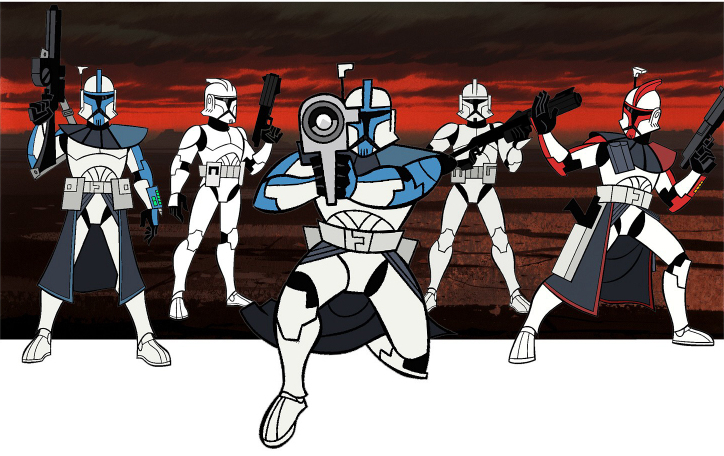
\includegraphics[width=0.75\textwidth]{img/clones}
    \end{column}
\end{columns}
}


\frame
{
\frametitle{Componentes}
\framesubtitle{Operador de Clonación}
\begin{itemize}
    \item Fórmula.

         $$m\ =\ \lceil\frac{\beta \cdot N}{a}\rceil$$
    \item Secuencia fija.
\end{itemize}
}

\frame
{
\frametitle{Componentes}
\framesubtitle{Operador de Reemplazo}
\begin{columns}
    \begin{column}{0.5\textwidth}
        \begin{itemize}
            \item Aleatorio.
            \item Peores.
        \end{itemize}
    \end{column}
    \begin{column}{0.5\textwidth}
        
\includegraphics[width=0.75\textwidth]{img/pregunta}
    \end{column}
\end{columns}
}


\frame
{
\frametitle{Componentes}
\framesubtitle{Movimiento}
\begin{columns}
    \begin{column}{0.5\textwidth}
        \begin{itemize}
            \item Swap 40\%.
        \end{itemize}
    \end{column}
    \begin{column}{0.5\textwidth}
        
\includegraphics[width=0.75\textwidth]{img/swap}
    \end{column}
\end{columns}
}

\frame
{
\frametitle{Componentes}
\framesubtitle{Configuraciones}
Normal:
        \begin{itemize}
            \item Generación de población: Cumpliendo restricciones duras.
            \item Selección de clones: Selección de los mejores.
            \item Reemplazo al término de iteración:  Se reemplazan los peores.
            \item Tipo de clonación: Mediante fórmula.
        \end{itemize}
}


\frame
{
\frametitle{Componentes}
\framesubtitle{Configuraciones}
Población Aleatorial:
        \begin{itemize}
            \item Generación de población: \blue{Rompiendo restricciones duras}.
            \item Selección de clones: Selección de los mejores.
            \item Reemplazo al término de iteración:  Se reemplazan los peores.
            \item Tipo de clonación: Mediante fórmula.
        \end{itemize}
}

\frame
{
\frametitle{Componentes}
\framesubtitle{Configuraciones}
Selección ruleta:

        \begin{itemize}
            \item Generación de población: Cumpliendo restricciones duras.
            \item Selección de clones: \blue{Selección mediante ruleta}.
            \item Reemplazo al término de iteración:  Se reemplazan los peores.
            \item Tipo de clonación: Mediante fórmula.
        \end{itemize}
}
\frame
{
\frametitle{Componentes}
\framesubtitle{Configuraciones}
Reemplazo aleatorio:

        \begin{itemize}
            \item Generación de población: Cumpliendo restricciones duras.
            \item Selección de clones: Selección de los mejores.
            \item Reemplazo al término de iteración:  \blue{Se reemplazan aleatoriamente}.
            \item Tipo de clonación: Mediante fórmula.
        \end{itemize}
}
\frame
{
\frametitle{Componentes}
\framesubtitle{Configuraciones}
Secuencia Fija:

        \begin{itemize}
            \item Generación de población: Cumpliendo restricciones duras.
            \item Selección de clones: Selección de los mejores.
            \item Reemplazo al término de iteración:  Se reemplazan los peores.
            \item Tipo de clonación: \blue{Secuencia fija}.
        \end{itemize}

}

